%% FC 2027 SHORT PAPER variant. Anonymized. LLNCS format.
%%
%% A separate submission from paper/fc27/, not a mode of it. The two are judged under
%% different CFP criteria -- the regular paper as a novel unpublished scientific
%% contribution, the short paper on novelty and potential to spark interest -- so they
%% are separate source trees built by one script (tools/build_fc27.py --target short)
%% from one set of generated figures and table fragments. The content budget is 8 pages
%% excluding references, no appendices of any kind, one figure, one table. The placebo
%% table was budgeted as a second table and released under D30; the comment at its former
%% position says what replaced it.
%%
%% Every numeric claim is carried verbatim from the regular version, whose printed claim
%% map remains the provenance record. The short version replaces that table with the
%% artifact URL, which is the one place its numbers can be traced.
\documentclass[runningheads]{llncs}
\usepackage{amsmath,amssymb}
\usepackage{graphicx}
\usepackage{booktabs}
\usepackage{array}
%% H2 T6. TikZ is loaded by the SHORT target only; paper/fc27/ does not use it and its
%% preamble is untouched. Figure 1 is drawn in TeX rather than imported as a PDF so the
%% schematic's type is the document's own and its sizes are the body's sizes.
%% positioning is not used by fig_schematic (which places by explicit coordinates) but
%% is loaded because figqa's standalone wrapper loads the same three libraries, and a
%% divergence there would mean the lane stops testing what the manuscript compiles.
\usepackage{tikz}
\usetikzlibrary{positioning,shapes.geometric,arrows.meta}
\PassOptionsToPackage{hyphens}{url}
\usepackage[hidelinks]{hyperref}
\Urlmuskip=0mu plus 1mu
\emergencystretch=1.5em

%% Byte-reproducible build, identical to the regular target's pins: pdfTeX draws the
%% PDF trailer's /ID from random bytes, so two builds of identical source otherwise
%% differ in hash. An empty \pdftrailerid{} fixes it; SOURCE_DATE_EPOCH (set by
%% tools/build_fc27.py) pins /CreationDate and /ModDate. Both are needed.
\pdftrailerid{}

%% Build-time width guard, same as the regular target: errors loudly instead of
%% silently overflowing into the margin if a regenerated fragment no longer fits.
\newlength{\tblw}
\newcommand{\checkwidth}[1]{\settowidth{\tblw}{#1}\ifdim\tblw>\textwidth\GenericError{}{TABLE TOO WIDE}{}{}\fi}

\begin{document}

%% D34. The "Short Paper:" prefix and its colon are CFP-mandated (recorded verbatim in
%% review/cfp_fc27_record.md); the CFP requires the title to BEGIN with that text. No
%% second colon, and sentence case after the prefix.
\title{Short Paper: What a disclosed reserve impairment cannot explain in the USDC
de-peg}
\titlerunning{Short Paper: What a disclosed impairment cannot explain}
\author{Anonymous Submission to FC 2027}
\authorrunning{Anonymous Submission}
\institute{}

\maketitle

\begin{abstract}
%% D35, H0's Variant N with the year restored. Narrative, one numeral (the year), and
%% the corollary deliberately absent. H0's draft joined two sentences with a semicolon;
%% split here, because the manuscript's punctuation rule bans semicolons in prose.
When an issuer publicly quantifies how much of its reserve is impaired while the
outcome is unresolved, that disclosure pins a worst-case floor under the coin's
value. We turn that into a reusable public-data instrument needing three
preconditions: the impairment is quantified while unresolved, the price falls
materially below par while the disclosure is live, and the fundamental channel is
reserve-only. Where the observed low breaches the floor, it returns a lower bound on
the part of the de-peg that expected loss cannot account for. Otherwise it returns no
verdict. Screening candidate episodes leaves one qualifying application, the March
2023 USD Coin de-peg, where the observed low does breach the floor. A cross-coin
placebo and three-episode panel sit outside the estimator. Because the residual covers
friction as well as panic, it speaks to backstop and redemption design rather than
reserve-quality rules alone.

\keywords{Stablecoins \and Bank runs \and De-peg \and Financial stability \and Market microstructure}
\end{abstract}

\section{Introduction}
\label{sec:intro}

Stablecoins are becoming payment infrastructure, and the GENIUS Act gives them their
first comprehensive U.S. federal framework~\cite{geniusact2025}. A fiat-backed stablecoin that
trades below par admits two readings. Under rational repricing, an impaired reserve
is worth less. Under non-fundamental repricing, a self-fulfilling coordination
run~\cite{diamonddybvig1983,goldsteinpauzner2005}
and microstructure friction push the price below the floor a reserve loss can justify. No
measurement of March 2023 cited in Section~\ref{sec:lit} forms that floor. A de-peg with
a non-fundamental share bounded away from zero calls for backstop and redemption design,
since a reserve-quality rule addresses only the fundamental share.

We offer a reusable estimator for any disclosed-impairment de-peg. From an issuer's
disclosed reserve impairment, derive a worst-case floor. Test whether the observed
trough breaches that floor. Read the breach, if any, as a bound on the non-fundamental
share. Figure~\ref{fig:schematic} shows those three steps. A supervisor can run it on any
public hourly print, within hours of a break. It returns no verdict when the trough does not
breach the floor.

%% H2 T6. Declared inside Section 1, immediately after the paragraph that cites it,
%% rather than in the skeleton between \input lines. A float is only considered from
%% its own position forward, and this is the earliest position that is still after its
%% first citation. The fragment is \input, not \includegraphics: it is a bare
%% tikzpicture with no figure environment of its own, so the wrapper lives here.
\begin{figure}[t]
\centering
\input{figures/fig_schematic}
\caption{The estimator. A disclosed impairment gives a floor, and a public price that
breaches it bounds the non-fundamental share.}
\label{fig:schematic}
\end{figure}

We apply it to the March 2023 USD~Coin (USDC) de-peg, where Silicon Valley Bank (SVB)
failed holding about $8\%$ of reserves, and a joint federal
backstop~\cite{fedtreasfdic2023pressrelease} restored the peg within days.

Under expected-loss pricing, fundamental value cannot fall below $1-\phi$, where $\phi$ is
the disclosed impairment fraction. Under (A4), a preference-free corollary extends that
floor to any monotone-utility valuation. The observed trough breaches the floor at every admissible
unremediated-loss probability and recovery rate, and requires $q^{\star}=1.54$, which
exceeds one. Under (A1)--(A3), no expected-loss account of the disclosed impairment is
consistent with the trough. At the disclosed $\phi$ the lower edge of the resulting
non-fundamental share runs from $19\%$ on Kraken's close to $35\%$ on the composite. It
stays positive across impairment readings, and at the full re-peg is $100\%$ ex post, an
identity
(Section~\ref{sec:ident}).

The paper makes two contributions:
\begin{itemize}
\item \textbf{An identification argument} (Proposition~\ref{prop:floor}) turning a
  disclosed impairment into a floor that a price either breaches or does not, with the
  breach read as a bound on the non-fundamental share.
\item \textbf{A screen} over six candidate de-pegs, none of which satisfies all three
  preconditions, so the single qualifying application is a property of the disclosure
  record rather than of the method.
\end{itemize}
Two analyses stay outside the estimator: the ex-ante fragility
ordering by reserve exposure that the realized troughs match, with null probability $1/2$
(Section~\ref{sec:placebo}), and a three-episode panel (Section~\ref{sec:spec}).

%% ============================================================================
\section{Related Work}
\label{sec:lit}

Since 2020 a literature applies run theory to stablecoin design and peg
arbitrage~\cite{Moin_2020,Klages_Mundt_2020,Lyons_2023,ahmed2025stablecoins}. Anadu et
al.~\cite{anadu2024} analyze the March 2023 de-peg through a discrete ``break-the-buck''
threshold. Watsky et al.~\cite{watsky2024}, and a later Federal Reserve
post-mortem~\cite{fedshadow2025}, attribute that break to a redemption window restricted
to Circle's approved customers over the March 10--13 weekend. Secondary prices de-pegged
while the arbitrage loop was closed. Uhlig~\cite{uhlig2022} finds many TerraUSD holders
behaved as rational Bayesian updaters in May 2022, evidence that rational and panic
behavior are hard to separate without a structural restriction.

Other work measures the March~2023 de-peg without an expected-loss floor: the SVB
link~\cite{galaticapalbo2023}, a daily cross-coin exposure ranking~\cite{diop2024fintech},
a detection lead of about five hours before USDC crosses
\$0.99~\cite{cintraholloway2023depegs}, a settlement-friction
framing~\cite{li2026settlementfriction}, and the on-chain contagion
pathway~\cite{sankaewtong2026contagion}. Our bound derives an expected loss from disclosed
exposure. None of the papers just cited does.

\noindent\textbf{Contribution boundary.} Structural calibrations~\cite{mzz2025} estimate a run
probability, and event studies~\cite{anadu2024} document flows. We bound one
episode's realized non-fundamental share from an accounting identity. Anadu et
al.'s~\cite{anadu2024} rational run concerns the redemption decision and makes no
claim about whether the price was justified. Watsky et al.'s~\cite{watsky2024} weekend
discount is the microstructure friction the non-fundamental share includes. Ahmed,
Aldasoro, and Duley~\cite{ahmedaldasoroduley2024} run synthetic-control tests on four
other episodes and treat March 2023 only as a price path.
Zhu~\cite{zhu2026redemptions} classifies which channel moves price and leaves
how far unmeasured. Molinet and Filos-Ratsikas~\cite{molinetfilos2026} define
fiat-backed coins as the always-stable case ($1/p_t=1$) and never analyze March 2023.
Eichengreen, Nguyen, and Viswanath-Natraj~\cite{Eichengreen_2025} back a devaluation
probability out of stablecoin prices, where the probability ours implies exceeds one.

%% ============================================================================
\section{Setting and Data}
\label{sec:setting}

%% C6. Compressed, but the arbitrage loop is NOT dropped: Section 2 uses the term
%% ("while the arbitrage loop was closed") and Section 1 does not define it, so cutting
%% the clause entirely would leave Section 2 resting on an undefined term.
USDC is a fiat-backed stablecoin redeemable one-for-one against Circle's
reserves of short-dated Treasuries and bank cash, so a bank failure impairs
backing through the cash leg and through the arbitrage loop of redemption at par.

Silicon Valley Bank failed on March~10, 2023. Late that evening, Circle
disclosed on its official X account that ``\$3.3 billion of the
${\sim}$\$40 billion of USDC reserves remain at SVB''~\cite{circle2023tweet}.
Circle restated that figure as ``about $8\%$'' of total reserves in its
March~12 press release~\cite{circle2023pressrelease}, and contemporaneous
reporting corroborates it~\cite{capoot2023}. We take $\phi\approx 0.08$,
Circle's own rounded disclosure. The
secondary-market price fell below par over March~10--11, reaching a trough of
\$0.877. On March~12 at 22:15~UTC, the FDIC, the Federal Reserve, and the
Treasury issued a joint statement guaranteeing SVB depositors in
full~\cite{fedtreasfdic2023pressrelease}, and USDC restored its peg over the
following days.

DAI, the contagion coin, is linked to USDC through MakerDAO's
peg-stability module, which swaps the two one-for-one up to a debt ceiling that
press reporting says was reached on 11~March 2023~\cite{theblock2023psm}.
Tether (USDT), the largest fiat-backed stablecoin, had no disclosed exposure to
SVB and serves as the unexposed coin.

All analysis runs offline on a frozen snapshot over the window 2023-03-08 to
2023-03-17 (UTC), and no proprietary data enters it. The headline USD price
series is an hourly cross-venue aggregate from the public aggregator
DeFiLlama~\cite{defillama2026api}. The
frozen record does not enumerate its constituent venues, so we do not treat it as an
independent venue. Kraken's fiat-settled USDC/USD close and
VWAP~\cite{kraken2026api} cross-check the \$0.877
trough, at minimum prints of \$0.901 and \$0.893. The pair's \$0.874 hourly low rests on
a single 3{,}373-USDC trade, so we do not read the cross-check off it. In
Figure~\ref{fig:event}(b) circles mark Kraken's close, drawn at its hour's end, and
triangles its VWAP, drawn at the midpoint.


%% Figure 1 is placed before the section that first cites it. LaTeX only considers a
%% float from its own position forward, so declaring it here is what lets it land on
%% Section 4's first page rather than drifting past the section that discusses it.
\begin{figure}[t]
\centering
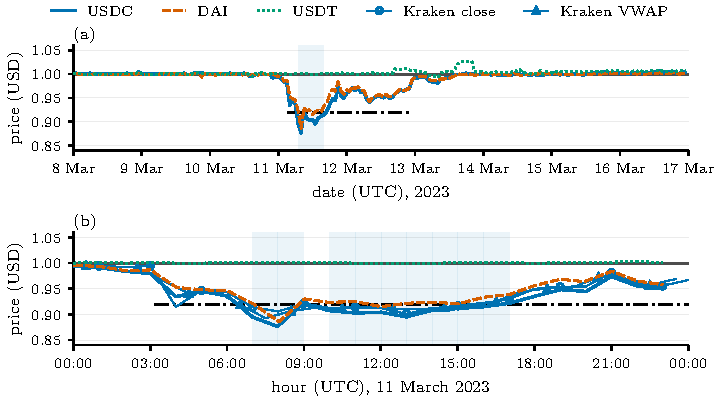
\includegraphics[width=\textwidth]{figs/fig_event_short.pdf}
%% D37. The reading instructions this caption used to carry now sit in the sections that
%% already state each underlying fact: the shading and the tenth hour in Section 4, the
%% Kraken markers in Section 3, the event lines in Section 5. The coin line styles
%% are dropped because figures.py draws a shared legend (add_shared_legend), so the
%% caption was restating the figure's own key.
\caption{Hourly USD prices of USDC, DAI and USDT over the window (a) and over
11~March 2023 (b), against par and the \$0.92 floor while the disclosure was live.}
\label{fig:event}
\end{figure}

%% ============================================================================
%% ============================================================================
\section{The Bound and Its Application}
\label{sec:ident}

The estimator is pure accounting, with no run threshold and no fitted parameter. Let
$\phi$ be the fraction of reserves impaired, $\rho\in[0,1]$ the expected recovery rate on
the impaired assets, and $q\in[0,1]$ the probability under the pricing measure that the
loss on the impaired fraction goes unremediated. Expected backing per coin is
\begin{equation}
P_{\mathrm{fund}}(q,\rho) = 1 - q\,\phi\,(1-\rho),
\end{equation}
and its minimum over $q$ and $\rho$, the worst-case floor, is $1-\phi$. The estimator
rests on three assumptions, and a fourth serves the preference-free argument below.

\begin{description}
\item[(A1) Reserve-only fundamental.] A coin's fundamental value is its expected reserve
  backing per unit given disclosed reserves, and the only impairment is the
  exposure $\phi$.
\item[(A2) Par redemption when solvent.] Conditional on rescue, redemption is at \$1
  within the frozen window.
\item[(A3) Bounded recovery.] Recovery on impaired reserves satisfies $\rho\in[0,1]$,
  because the coin is fully reserved and the reserves carry no leverage.
\item[(A4) Monotone-utility valuation.] The unconstrained marginal holder values the claim
  as an expected utility of its payoff, for some monotone increasing utility and some
  probability measure over outcomes, with no ambiguity about the disclosed $\phi$. This nests risk neutrality, any degree of risk
  aversion, and rank-dependent weighting.
\end{description}

\begin{proposition}[Rational-pricing floor and impossibility]
\label{prop:floor}
Assume \textup{(A1)--(A3)}. Then
$P_{\mathrm{fund}}(q,\rho)\in[\,1-\phi,\,1\,]$ for all $q,\rho\in[0,1]$, so no expected
loss on the disclosed impairment justifies a value below $1-\phi$. The unremediated-loss
probability an observed price $P_{\mathrm{obs}}<1-\phi$ would require, at the worst-case
recovery $\rho=0$, is $q^{\star}=(1-P_{\mathrm{obs}})/\phi>1$.
\end{proposition}

\begin{proof}
$P_{\mathrm{fund}}$ is decreasing in $q$ and increasing in $\rho$, so it is minimized at
$(q,\rho)=(1,0)$ at value $1-\phi$ and maximized at $q=0$ at value $1$, and $q^{\star}$
solves $P_{\mathrm{obs}}=1-q\phi$ at $\rho=0$. \qed
\end{proof}

This is the floor-at-recovery-value bound of credit
pricing~\cite{merton1974,duffiesingleton1999}.

Under (A1)--(A4) the floor is also preference-free. By (A2) and (A3) the payoff $X$ on a
USDC claim has support in $[1-\phi,1]$ in every state. For any monotone increasing utility
$u$, the certainty equivalent $u^{-1}\!\bigl(\mathbb{E}[u(X)]\bigr)$ of a lottery with
that support lies in $[1-\phi,1]$ as well. That floor bounds rational
valuations, meaning willingness to pay. It does not bound market-clearing
prices, because a seller under binding margin or capital constraints can rationally
transact below every unconstrained valuation~\cite{shleifervishny1997,grombvayanos2010}.
That channel is a friction, and the non-fundamental share defined next includes it. The
floor is only as strong as the support condition $X\in[1-\phi,1]$, which does not cover
issuer-wrapper risk~\cite{Gorton_2021}.

Write the observed deviation $1-P_{\mathrm{obs}}$ and the fundamental deviation
$\phi(1-\rho)$. The non-fundamental share of the de-peg is
\begin{equation}
s_{\mathrm{nf}}(\rho)
  = \frac{(1-P_{\mathrm{obs}})-\phi(1-\rho)}{1-P_{\mathrm{obs}}} .
\label{eq:share}
\end{equation}
Its lower edge takes $\rho=0$, treating total permanent loss of the impaired reserves as
the fundamental cap. Its upper edge takes $\rho=1$, the full re-peg, which
implies zero permanent loss and gives $s_{\mathrm{nf}}(1)=1$, or $100\%$ ex post, an
identity. The residual covers coordination panic and microstructure friction together, so
the share is an upper bound on pure coordination panic.

With the disclosed impairment $\phi=0.08$, the worst-case floor is $1-\phi=\$0.92$ and the
observed trough is $P_{\mathrm{obs}}=\$0.877$.\footnote{Prose rounds troughs to three figures.
Computation uses the frozen four-figure print, so \$0.877 enters as $0.8767$ and
Section~\ref{sec:placebo}'s deviations reconcile at full precision.} The trough lies below the floor, so under
(A1)--(A3) no expected loss rationalizes it, and the implied unremediated-loss probability
is $q^{\star}=(1-0.877)/0.08=1.54$. The lower edge of
\eqref{eq:share} is
$(0.1233-0.08)/0.1233=0.351$, so at least $35\%$ of the de-peg is non-fundamental. Across three
readings of Circle's disclosure and five trough readings across four feeds, the fifth
being the composite's second-lowest print, the lower edge runs from
$16.7\%$ to $36.4\%$, and every one of those fifteen combinations breaches the floor. At
the disclosed $\phi$, the lowest is $19.2\%$, from Kraken's close, whose minimum print
is \$0.901. By
Proposition~\ref{prop:floor} the trough is unrationalizable for any impairment below
$12.3\%$, a $4.3$-point margin over the disclosed $8\%$, and the lower edge stays strictly
positive across that margin. Figure~\ref{fig:share} plots that edge against $\phi$ for
the composite, Kraken close and VWAP troughs, each crossing zero at the impairment
that would make its own trough rationalizable.

%% H2 T6. Declared AFTER the paragraph that cites it, not before. The PDF is copied
%% into figs/ by tools/build_fc27.py's sync_figs step, which is driven by the
%% \includegraphics targets in this tree, so naming it here is what brings it across;
%% it is never hand-copied.
%% Placement: a float is only considered from its declaration forward. Declared
%% BEFORE this paragraph it reached page 5 while the citing sentence landed on page
%% 6, so the figure appeared before the page that first cites it. Declaring it here
%% makes page 6 the earliest page it can reach.
\begin{figure}[t]
\centering
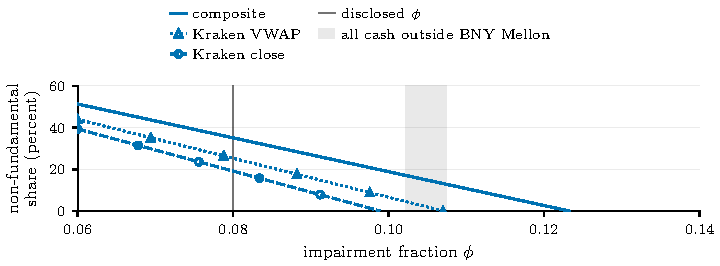
\includegraphics[width=\textwidth]{figs/fig_share_vs_phi.pdf}
\caption{Lower-edge non-fundamental share against impairment. Curves cross zero at one
minus their troughs. Shading treats cash outside BNY Mellon as impaired.}
\label{fig:share}
\end{figure}

Under (A1), $\phi$ is Circle's disclosed figure, and evaluating at $\rho=0$ uses the
lowest floor (A3) allows. Against the circulating supply at the trough, which exceeds
the \$40B figure Circle used, $\phi$ is $0.079$, below the headline $0.08$.

Circle's disclosure quantifies only the SVB deposit, but the same update itemizes the
whole cash leg: \$9.7B, of which \$5.4B sat at BNY Mellon, \$3.3B at SVB and \$1B at
Customers Bank, with no exposure to Silvergate~\cite{circle2023update}. With the \$32.4B
Treasury leg the same update reports, reserves total \$42.1B. Treating all cash outside
BNY Mellon as impaired gives $\phi=0.102$ on that total, where the
lower edge is $17.2\%$ on the composite and $4.7\%$ on Kraken's VWAP and Kraken's close
returns no verdict. On the \$40B base the same reading gives $\phi=0.1075$, where only
the composite still returns a verdict, at $12.8\%$.

Kraken's $240$ hourly bars run one day longer than the composite's $216$-hour window,
in which four snapshots are absent, and against that denominator its close breaches the
\$0.92 floor in 9 hours, its VWAP in 10, and its hourly low in 12. Sub-floor trades
themselves fall in twelve clock hours, $37{,}303$ of them worth \$154.0M.

Because the estimator needs only a price and a publicly quantified $\phi$, it can be
evaluated at every hour of the frozen window (Figure~\ref{fig:event}). Of USDC's $212$
in-window hourly readings, $9$ lie below the \$0.92 floor, and all nine fall on 11~March
2023 between 06{:}59 and 16{:}00~UTC, shaded in both panels. The
tenth hour of that window, at 08{:}57, recovers to \$0.9216. That impossibility window measures duration and
specificity. It adds no evidence volume, because hourly prices within one episode are
near-unit-root, with lag-1 autocorrelation $r=0.963$, so the $212$ readings carry an
AR(1)-adjusted effective sample size $n(1-r)/(1+r)=4.0$. The lower edge, $q^{\star}$, and the
floor-breach indicator are three readings of $1-P_{\mathrm{obs}}-\phi$, so their agreement
corroborates nothing.


%% The cross-stablecoin placebo table is generated (tables/tab_placebo_short.tex) but NOT
%% placed. It was the third float in an eight-page budget, and releasing it was the single
%% largest page saving available: nine lines, measured. Nothing it printed is lost.
%% Section 5's prose now carries all three troughs, all three basis-point deviations, both
%% USDT premium peaks with the later one labelled post-backstop, and the break outcome for
%% each coin, along with the precision note the caption carried. The fragment stays in the
%% repository so the table can be restored if the page budget ever allows it.
%%
%% The sensitivity grid is generated (tables/tab_sens_short.tex) but NOT placed. Two
%% reviewers asked for the fifteen-number Section 4 paragraph to become a table, and
%% one predicted the table would SAVE space. It did not: as a fourth float with its own
%% caption it cost about twelve lines net, against a paper already at its page limit.
%% The paragraph it replaced is gone either way, which was the reviewers' actual
%% complaint, and Section 4 now states the range, the extreme cell and its feed in
%% prose. The fragment stays in the repository so the grid can be restored if the page
%% budget ever allows it.

%% The three-episode table is generated (tables/tab_panel_short.tex) but NOT placed.
%% D42-A released it, on D30's precedent and for D30's reason: it was the last float in an
%% eight-page budget and releasing it was the only remaining saving large enough to close
%% the gate. Measured, not estimated: 23 lines, which moved the last line of Section 7 from
%% page 9 line 19 to page 8, and it is the only change that did. The three earlier rungs of
%% H2's ladder returned 5 lines between them.
%%
%% Nothing it printed is lost. Section 6's prose now states all three episodes in order,
%% each with the disclosure source, phi, floor, trough and feed, q-star, and the fire /
%% no-verdict outcome. The footnote marks [a] and [b] are gone with the table; their text
%% ("regulator-quantified, issuer-contested" and "degenerate by construction") was already
%% in Section 6's prose before the release, so nothing had to be carried across for them.
%%
%% The fragment stays in the repository, unreferenced by this manuscript, because the
%% journal leg reuses it and because the table can be restored if the page budget ever
%% allows it. With this release the short paper has no table at all, which is why the
%% verification sweep greps the built PDF for the word "Table" and expects zero hits.

%% ============================================================================
\section{Cross-Coin Evidence}
\label{sec:placebo}

Reserve exposure orders the three coins ex ante: USDC held direct SVB exposure, DAI was
pinned to USDC through the peg-stability module, and USDT held none. That gives
the ex-ante fragility ordering USDC, DAI, USDT. Troughs are \$0.877, \$0.886, and
\$0.992 in that order. The deviations from par are $1233$, $1141$, and $76$~bps.
DAI's mechanical link to USDC leaves one free
comparison, so the realized ordering has probability $1/2$ and illustrates the ex-ante
ordering without testing it. USDC and DAI clear the $1\%$
break threshold, a deviation of at least one cent from par, by factors of
$12$ and $11$. USDT does not clear it, so the placebo criterion is satisfied: the
exposed coins break and the unexposed coin does not.

\noindent\textbf{USDT as the unexposed control.} USDT was bid to a premium while USDC and
DAI fell. That pattern is consistent with the crypto safe-haven behavior documented for
USDT~\cite{Baur_2021}. The premium is venue- and time-specific. On Coinbase
\texttt{USDT-USD}~\cite{coinbase2026exchangeapi} it peaked at $+266$~bps at 02:00~UTC on
11~March, 71 minutes before
Circle's 03:11~UTC disclosure. Over the window \$1.24B of \$1.52B traded above par, and
that peak is one hour of it. The composite feed peaks later and higher, at $+270$~bps at
19:00~UTC on 13~March. That peak falls after the joint federal backstop of the previous
evening, so it is post-backstop rather than intra-run. The
Coinbase premium responds to the SVB failure itself, because Circle's
USDC-specific disclosure had not yet been made. A
common-factor repricing of stablecoin risk would move all three coins down
together, so it cannot produce that premium. Rational substitution out of a gated
claim can, and the two are not separated here.

\section{Screening}
\label{sec:spec}

The estimator requires three preconditions. First~(i), $\phi$ must be publicly
quantified while the exposure is unresolved. Second~(ii), the price must fall more
than $1\%$ below par while that disclosure is live. Third~(iii), the fundamental
channel must be reserve-only, so that $1-\phi$ is the floor. Beyond the application
itself and Tether~(2019), we screened six candidate episodes: BUSD, Tether~(2022),
USDR, USDP, GUSD, and TUSD. None satisfies all three, and each fails in one of two
ways: no disclosed impairment, or a loss measured under a different valuation model.
Issuers with a material impairment did not disclose its size in any of the six, so one
qualifying episode is a property of the disclosure record.

Three episodes bound the estimator's behavior: the qualifying application in
USDC~(2023), and two that return no verdict, Tether~(2019) and Tether~(2022), which is
USDT over the Terra episode of May 2022~\cite{liumakarovschoar2023}. USDC fires on Circle's 03{:}11~UTC disclosure of
11~March~\cite{circle2023tweet}: $\phi=0.08$, floor \$0.92, composite headline trough
\$0.877 at 07{:}57~UTC, and $q^{\star}=1.54$. Tether's episode is assessed under
precondition~(i). The New York Attorney General's 25~April 2019
statement~\cite{nyag2019tether} quantified Tether's exposure and Tether contested the
characterization. The statement implies
$\phi\in[0.2585,\allowbreak 0.3324]$ and a floor in $[0.6676,\allowbreak 0.7415]$. The deepest post-disclosure Kraken USDT/USD print, \$0.9551
on 26~April 2019, is 21.4 to 28.8 cents above every worst-case floor, and
$q^{\star}\in[0.135,0.174]$, so the verdict is no verdict, above floor.
We read both
episodes at zero recovery on the impaired reserves, so the same one-sided bound
governs both. Tether~(2022) has no disclosure, so $\phi=0$ and
precondition~(i) fails. The floor would be par, which any sub-par print breaches as an
identity and not as evidence, so the verdict is no verdict, undisclosed.

Read strictly, precondition~(i) demands the issuer's own public quantification while
the exposure is unresolved, and under that reading the panel contains no validated
true negative. One episode on which the bound returns no verdict does not measure a
false-positive rate. The specificity of the bound is unmeasured, and unmeasurable on the
current record, because a validated true negative needs an issuer-disclosed $\phi$ whose
trough stays above $1-\phi$, and no screened episode supplies one.

TrueUSD's unremediated impairment during our window was not publicly quantified until a
September 2024 SEC complaint~\cite{sectruecoin2024}, so precondition~(i) fails and the
verdict is again no verdict, undisclosed. The residual is defined relative to
what the market could know, because a concealed impairment produces no signal.

\section{Limitations and Conclusion}
\label{sec:conc}

The panic-versus-fundamentals split is contested~\cite{anadu2024,watsky2024}. The
composite feed could mismeasure the trough. The disclosed $\phi$ could understate
exposure. The breakeven impairment is $12.3\%$ on the composite and $9.9\%$ on Kraken's
close, and the
worst case the disclosure admits, $\phi=0.102$, sits between them. A time-value discount
prices a delayed
redemption for a holder who has an approved claim. Convertibility risk is the cost to a
holder without an approved claim during the restricted window. That cost is not bounded
by the discount and belongs to the residual. No public data source can bound it further. We identify the mechanism from a
single episode. The ex-post $100\%$ is an aggregate statement, and holders who sold
at the trough still realized losses.

%% The identifier is wrapped in its own \mbox so it cannot break across a line. url's
%% hyphens option lets a URL break at any hyphen, which here rendered
%% "usdcdepeg-artifact" across a break and read as a different identifier. The \mbox
%% costs no line: the prefix still breaks after "/r/". No trailing slash, matching the
%% registered URL.
%% Two \url calls emit TWO link annotations, and the second one targets the bare
%% identifier as a relative reference, so clicking it does not reach the artifact. One
%% \href carrying the whole address wraps both \nolinkurl pieces in a single annotation,
%% and \nolinkurl keeps the url typography and breakpoints without adding a link of its
%% own.
%% The URL sits at the END of its sentence, which is what keeps the gate clean. Prefix
%% plus boxed identifier is about 304pt and fits a 347pt line ALONE, but not after a
%% leading "An anonymized artifact at" (about 118pt). With the URL leading the sentence
%% every interior breakpoint of the prefix left a first line too short to fill, so TeX
%% preferred an overfull box and the build gate failed at 88.3pt. \allowbreak at the
%% seam does not fix that; only letting the URL start a fresh line does.
The frozen snapshot, the seeded analysis code, and a manifest with a SHA-256 digest for
every file it lists sit in an anonymized artifact at
\href{https://anonymous.4open.science/r/usdc-depeg-artifact-fc27}%
{\nolinkurl{https://anonymous.4open.science/r/}\mbox{\nolinkurl{usdc-depeg-artifact-fc27}}}.
Every computed number and figure regenerates offline from the
artifact without an API key.

A disclosed impairment implies a worst-case floor, and the USDC trough lies below it.
Under (A1)--(A3) and at the disclosed $\phi$, at least $35\%$ of the de-peg was non-fundamental by impossibility on the composite feed, and at least $19\%$ on Kraken's
close, the most conservative feed. At the worst case the disclosure itself admits,
$\phi=0.102$, the composite still returns a verdict and Kraken's close does not.
Whether that residual is coordination panic or
convertibility friction on a closed redemption rail, both point to backstop and redemption
design rather than reserve-quality rules alone, so the policy reading does not depend on
the split. The estimator needs only a price and a publicly quantified $\phi$.


\bibliographystyle{splncs04}
\bibliography{refs}

\end{document}
